\chapter{\iflanguage{ngerman}{Zukünftige Entwicklung}{Development}}
\label{sec:overview}

In Science Fiction Filmen wie Transcendence wird die Zukunft des Operationssaals gerne mit vollautomatisierten Robotersystemen dargestellt, die innerhalb von wenigen Sekunden komplexe Eingriffe durchführen können. 
Mit welchen Entwicklungen aber tatsächlich in naher Zukunft gerechnet werden kann und welche Sci Fi Ideen gar nicht so weit von der Wirklichkeit entfernt sind, soll in den folgenden Abschnitten erläutert werden.

\subsection{Neue Technologien}
Neue Technologien haben das Ziel, die Möglichkeiten im OP zu erweitern, mehr Sicherheit bzw. ein geringeres Risiko zu gewährleisten und das Team bei schwierigen Aufgaben zu unterstützen \cite{CurrentAndFuture}. 

Durch die Verbesserung der Bildqualität von Ultraschall (US) wird dieser in naher Zukunft vermehrt in OP-Sälen anzutreffen sein. Neue Möglichkeiten, wie der Aufnahme von dreidimensionalen Objekten (siehe Abb. \ref{fig:us}) in Echtzeit, eröffnen noch nicht dagewesene Anwendungsgebiete \cite{BrainShiftInTumorResection}. Hinzu kommen Möglichkeiten für die intravaskuläre Bildgebung, zur Aufnahme von Gefäßwänden mit an Kathetern befestigten US-Köpfen. Der Vorteil von US ist, dass gegenüber anderer Bildgebender Verfahren, weder der Patient noch das behandelnde Team radiologischer Strahlung ausgesetzt werden \cite{CurrentAndFuture}. Aus diesen Gründen und einer relativ guten Korrelation zwischen US- und MR-Bildern, wird US auch in der Neuronavigation Anwendung finden \cite{BrainShiftInTumorResection}. \\
Bisher ist der Einsatz von Roboter- und Navigationssystemen im veränderlichen Körper begrenzt einsetzbar \cite{DerDigitaleOperationssaal}. Doch neue Funktionen wie Instrumentennavigation, Kollisionswarnungen und Neuromonitoring ermöglichen strahlenfreie Mikromanipulation, Navigation und Instrumentenführung. Besonders bei langen komplexen Operationsvorgängen versprechen diese mehr Sicherheit und Kontrolle \cite{DerDigitaleOperationssaal,CurrentAndFuture}. \\
Bei derzeit in der Medizintechnik eingesetzten Robotersystemen handelt es sich meist um Master-Slave-Systeme. Also Systeme die vom Menschen gesteuert werden und mit denen bei komplexen Eingriffen über kleine Zugänge präzise gearbeitet werden kann. Aufgrund der vergleichsweise hohen Investitionskosten werden Robotersysteme in erster Linie für Eingriffe entwickelt, die der Chirurg ohne nicht ausführen könnte \cite{DerDigitaleOperationssaal}. Wie für das Operieren über natürliche Körperöffnungen. Erste Versuche wurden bereits mit dem Endosamurai (siehe Abb. \ref{fig:endosamurai}) der Olympus Deutschland GmbH durchgeführt. Gegenüber Konventioneller Endoskope können mit dem Endosamurai über einen Zugang mit den Instrumentenarmen Zug- und Gegenkräfte aufgebracht werden \cite{Endosamurai,DerDigitaleOperationssaal}. 

Hinzu kommt eine standardisierten Vernetzung der Geräte und Systeme und herstellerübergreifende Kombinationslösungen. Ein übersichtliches Interface und zusätzliche Sprachsteuerung sollen zur Optimierung des chirurgischen Workflows beitragen. Die weitere Entwicklung in der computergestützten Optimierung der Visualisierung erlaubt zukünftig kontinuierliche Aufzeichnungen des Eingriffs \cite{DerDigitaleOperationssaal}. Daraus können Informationen zur automatisierten Operationsplanung für die individuelle Anatomie des Patienten gewonnen werden \cite{CurrentAndFuture}.

\begin{figure} [H]
	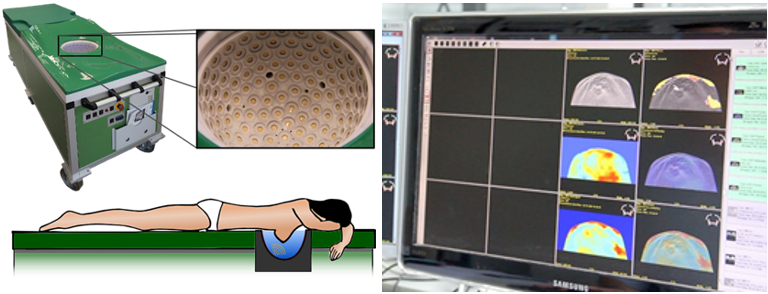
\includegraphics[scale = 0.5]{Content/Pictures/us.png}
	\caption{(Links) Wassergefülltes Untersuchungsbecken für eine (rechts) dreidimensionale Ultraschallaufnahme von der Brust zur Brustkrebsfrüherkennung \cite{Ultraschall}.} 
	\label{fig:us}
\end{figure}

\begin{figure} [H]
	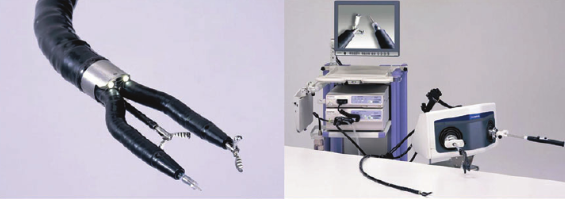
\includegraphics[scale = 0.7]{Content/Pictures/endosamurai.png}
	\caption{Endosamurai von der Olympus GmbH \cite{EndosamuraiBild}.} 
	\label{fig:endosamurai}
\end{figure}

\subsection{Ausblick}
Wie sich der Operationssaal zukünftig entwickeln wird und welche Technologien von den theoretisch möglichen umgesetzt werden ist abhängig von den wirtschaftlichen Realitäten. Unabhängig davon, ist ein eindeutiger Trend in Richtung minimalinvasive Eingriffe zu verzeichnen. Dieser Trend wird durch die Entwicklungen in der Mikro- und Nanotechnik unterstützt und ermöglicht immer geringer belastendere Eingriffe \cite{DerDigitaleOperationssaal}. 

Monoport-Techniken und narbenlose Operationsverfahren über natürliche Körperöffnungen gewinnen zunehmend an Bedeutung. Zur Umsetzung dieser Entwicklung, müssen miniaturisierte Telemanipulationssysteme eingesetzt werden. Beispielsweise könnten autonome kabelgeführte Miniroboter über einen kleinen Zugang in den Körper eingeführt werden und sich selbständig zu einer bestimmten Position im Körper vorarbeiten. So könnte der Chirurg die schwierige Navigation durch den Körper abgeben und durch den Einsatz von am Katheter angebrachter miniaturisierte Visualisierungssysteme den Vorgang überwachen \cite{DerDigitaleOperationssaal}.\\
Eine andere vorstellbare Entwicklung könnte in Richtung eines minimierten Reinraums gehen. Dabei könnte in einer unsterilen Umgebung ein mit Vakuum fixierter Aufsatz über die Oberfläche des \glqq point of interest\grqq{} gestülpt und die Instrumente über einen Schleuse hindurchgeführt werden. Zur Umsetzung dieser Vision werden dann individualisierte \glqq single use\grqq{} Instrumente angefertigt und garantieren so eine optimale Abstimmung auf den Patienten und die Aufgabenstellung \cite{DerDigitaleOperationssaal}.
%In vielen Fällen kommt der Chirurg bei einer Operationen an die Grenzen seiner menschlichen Konzentrationsfähigkeit, da %teilweise mit Händen und Füßen die medizinischen Geräte gesteuert werden müssen. Aus diesem Grund wird bereits die %Sprachsteuerung integriert aber darüber hinaus ist eine Steuerung beispielsweise über die Augen vorstellbar. So könnte der %Chirurg sein medizinisches Umfeld manipulieren ohne seine Körperposition zu ändern und beispielsweise bestimmte Ausschnitte %des Patienten beliebig vergrößern oder verkleinern. Genauso könnte direkte Abstandsmaße von anatomischen Gegebenheiten %genommen und angezeigt werden \cite{DerDigitaleOperationssaal}. \\



Die Mensch-Maschine-Interaktion spielt eine immer wichtigere Rolle und in der Zukunft wird das Zusammenspiel aus Bildgebenden Verfahren, Navigation, Robotik, IT und Benutzerinteraktion perfektioniert \cite{CurrentAndFuture}.
Auch heute schon ist der Hybride OP-Saal die Zukunft der Chirurgie \cite{Maquet}. Das wird sowohl den Patienten als auch den Chirurgen und dem Team zu Gute kommen.


	
	



